
\chapter{Analisi dei requisiti}
\label{cap:analisi-requisiti}

\section{Casi d'uso}

In questo capitolo si illustrano i vari casi d'uso per il progetto ENGaming.\\
Per lo studio dei casi d'uso vengono utilizzati dei diagrammi, chiamati diagrammi dei casi d'uso (in inglese \emph{Use Case Diagram}).
Questi diagrammi sono diagrammi \gls{umlg}, dedicati alla descrizione delle funzioni offerte da un applicativo, descrivendoli come sono percepiti e utilizzati dagli attori che interagiscono col sistema stesso.

\subsection{Attori}

Essendo questo prodotto rivolto agli utenti finali, l'unico attore presente nei casi d'uso è l'utente.
Non viene fatta una distinzione tra un utente generico e un utente autenticato poichè non viene previsto che l'applicativo implementi un sistema di autenticazione.

\begin{figure}[h]
    \centering
    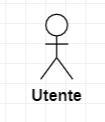
\includegraphics{images/usecase/attore.png}
    \caption{Attore presente nei casi d'uso}
    \label{fig:attore}
\end{figure}
\newpage
\subsection{UC01 - Visualizzazione schermata iniziale}
\begin{figure}[h]
    \centering
    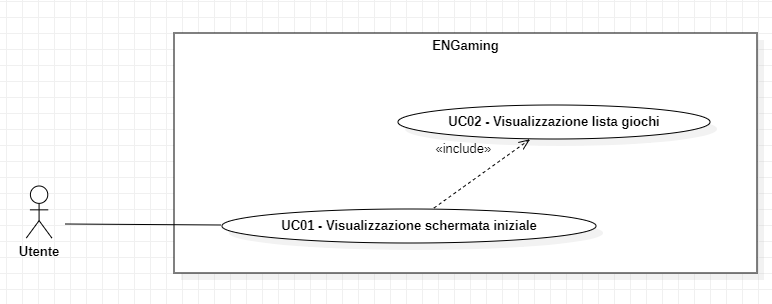
\includegraphics[width=400pt]{images/usecase/UC01.png}
    \caption{Diagramma dei casi d'uso per la schermata iniziale}
    \label{fig:UC01}
\end{figure}
\begin{itemize}
    \item Attore principale: Utente
    \item Pre-condizioni: l'utente non visualizza la schermata iniziale.
    \item Post-condizioni: l'utente visualizza la schermata iniziale.
    \item Scenario principale: \begin{itemize}
        \item Il sistema carica l'applicazione sul device ENSign11.
        \item L'utente arriva nella postazione in cui è presente il device.
        \item L'utente visualizza, sullo schermo del device, una lista di giochi selezionabile e un pulsante relativo ai record.
    \end{itemize}
    \item Include: \begin{itemize}
        \item UC02 - Visualizzazione lista giochi
    \end{itemize}
\end{itemize}
\newpage
\subsection{UC02 - Visualizzazione lista giochi}
\begin{figure}[h]
    \centering
    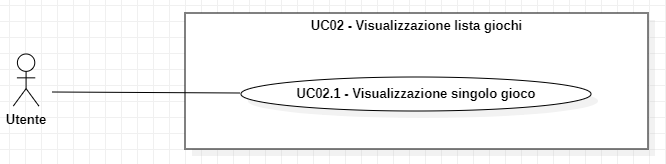
\includegraphics[width=400pt]{images/usecase/UC02.png}
    \caption{Diagramma dei casi d'uso per la visualizzazione della lista dei giochi}
    \label{fig:UC02}
\end{figure}
\begin{itemize}
    \item Attore principale: Utente
    \item Pre-condizioni: l'utente non visualizza la lista dei giochi disponibili.
    \item Post-condizioni: l'utente visualizza la lista dei giochi disponibili.
    \item Scenario principale: \begin{itemize}
        \item L'utente visualizza una lista di giochi selezionabili. La lista è composta da icone che possono essere selezionate tramite il tocco. Essendo visualizzabili al massimo dieci icone relative ai giochi, l'utente può utilizzare gli appositi pulsanti per visualizzare le icone non visibili.
    \end{itemize}
    \item Include: \begin{itemize}
        \item UC02.1 - Visualizzazione singolo gioco
    \end{itemize}
\end{itemize}

\subsection{UC02.1 - Visualizzazione singolo gioco}
\begin{figure}[h]
    \centering
    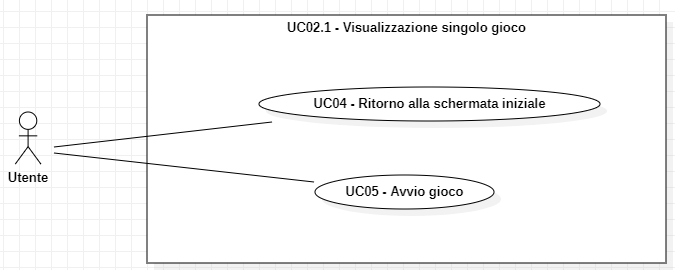
\includegraphics[width=400pt]{images/usecase/UC02_1.png}
    \caption{Diagramma dei casi d'uso per la visualizzazione di un singolo gioco}
    \label{fig:UC02.1}
\end{figure}
\begin{itemize}
    \item Attore principale: Utente
    \item Pre-condizioni: l'utente sta visualizzando la lista dei giochi disponibili.
    \item Post-condizioni: l'utente visualizza le caratteristiche del singolo gioco.
    \item Scenario principale: \begin{itemize}
        \item L'utente, dalla lista di giochi selezionabili, seleziona un gioco.
        \item L'utente viene reindirizzato nella pagina del gioco scelto. Ogni gioco contiene, oltre all'apposito pulsante per iniziare a giocare, le seguenti informazioni: \begin{itemize}
            \item Nome del gioco
            \item Tipo di gioco (es. arcade, racing, action...)
            \item Descrizione del gioco, se presente
            \item Tipologia d'input, tra controller e touch/digitalizer
            \item Mappatura dei comandi, se il gioco richiede l'uso del controller
        \end{itemize} Inoltre, la pagina contiene anche un pulsante per tornare alla schermata iniziale.
    \end{itemize}
    \item Include: \begin{itemize}
        \item UC04 - Ritorno alla schermata iniziale
        \item UC05 - Avvio gioco
    \end{itemize}
\end{itemize}
\newpage
\subsection{UC03 - Visualizzazione record}
\begin{figure}[h]
    \centering
    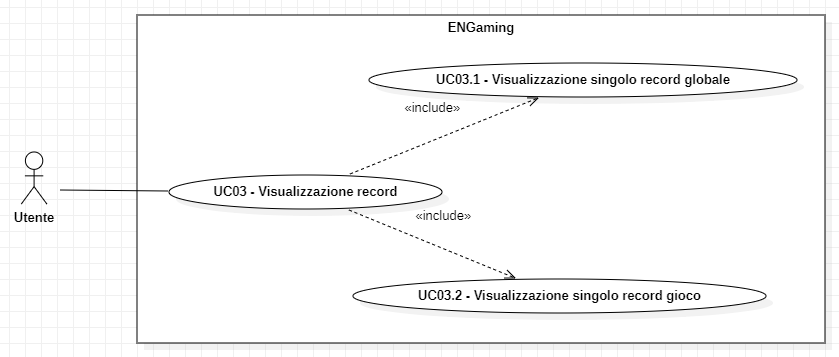
\includegraphics[width=400pt]{images/usecase/UC03.png}
    \caption{Diagramma dei casi d'uso per la visualizzazione dei record}
    \label{fig:UC03}
\end{figure}
\begin{itemize}
    \item Attore principale: Utente
    \item Pre-condizioni: l'utente si trova nella schermata principale, e non sta visualizzando i record.
    \item Post-condizioni: l'utente visualizza i record.
    \item Scenario principale: \begin{itemize}
        \item L'utente preme il pulsante relativo ai record, posto nell'area principale.
        \item L'utente, in una nuova pagina, visualizza la lista dei record globali, ovvero di tutti i record presenti nel device, ordinati per punteggio. In caso di punteggio uguale, i record vengono ordinati per data ed eventualmente per nome del gioco ascendente.
        \item L'utente, tramite gli appositi pulsanti, rimane nella stessa pagina e può passare alle liste per gioco, visualizzando i record presenti per i singoli giochi, ordinati per punteggio. In caso di punteggio uguale, i record vengono ordinati per data.
    \end{itemize}
    \item Include: \begin{itemize}
        \item UC03.1 - Visualizzazione singolo record globale
        \item UC03.2 - Visualizzazione singolo record gioco
    \end{itemize}
\end{itemize}

\subsection{UC03.1 - Visualizzazione singolo record globale}
\begin{itemize}
    \item Attore principale: Utente
    \item Pre-condizioni: l'utente sta visualizzando la lista dei record globali.
    \item Post-condizioni: l'utente visualizza le caratteristiche del singolo record.
    \item Scenario principale: \begin{itemize}
        \item L'utente, dalla lista dei record presenti, ne vede i dettagli. Ogni record nella lista globale contiene le seguenti informazioni: \begin{itemize}
            \item Posizione in classifica
            \item Nome dell' utente che ha effettuato il record, composto da tre lettere
            \item Punteggio conseguito
            \item Nome del gioco in cui si è fatto il record
        \end{itemize}
    \end{itemize}
\end{itemize}

\subsection{UC03.2 - Visualizzazione singolo record gioco}
\begin{itemize}
    \item Attore principale: Utente
    \item Pre-condizioni: l'utente sta visualizzando la lista dei record per un determinato gioco.
    \item Post-condizioni: l'utente visualizza le caratteristiche del singolo record.
    \item Scenario principale: \begin{itemize}
        \item L'utente, dalla lista dei record presenti, ne vede i dettagli. Ogni record nella lista di un determinato gioco contiene le seguenti informazioni: \begin{itemize}
            \item Posizione in classifica
            \item Nome dell' utente che ha effettuato il record, composto da tre lettere
            \item Punteggio conseguito
        \end{itemize}
    \end{itemize}
\end{itemize}

\subsection{UC04 - Ritorno alla schermata iniziale}
\begin{itemize}
    \item Attore principale: Utente
    \item Pre-condizioni: l'utente vuole tornare alla schermata iniziale.
    \item Post-condizioni: l'utente si trova nella schermata iniziale.
    \item Scenario principale: \begin{itemize}
        \item L'utente preme l'apposito pulsante per ritornare nella schermata iniziale.
        \item Il sistema riceve l'input dal device e reindirizza l'utente verso la schermata iniziale.
    \end{itemize}
\end{itemize}

\newpage
\subsection{UC05 - Avvio gioco}
\begin{figure}[h]
    \centering
    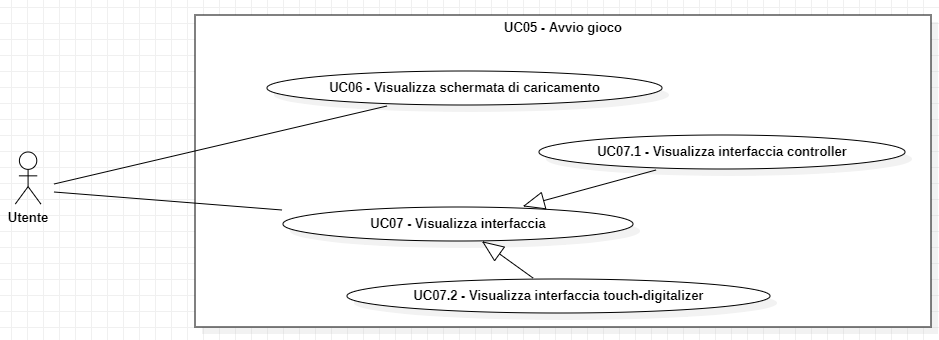
\includegraphics[width=400pt]{images/usecase/UC05.png}
    \caption{Diagramma dei casi d'uso per l'avvio di un gioco}
    \label{fig:UC05}
\end{figure}
\begin{itemize}
    \item Attore principale: Utente
    \item Pre-condizioni: l'utente sta visualizzando le caratteristiche del singolo gioco.
    \item Post-condizioni: l'utente è pronto per giocare.
    \item Scenario principale: \begin{itemize}
        \item L'utente, che si trova nella schermata di un gioco, avvia il gioco tramite l'apposito pulsante.
        \item L'utente visualizza una pagina di caricamento.
        \item Al termine del caricamento, l'utente visualizza una pagina con il gioco e l'interfaccia necessaria.
    \end{itemize}
    \item Include: \begin{itemize}
        \item UC06 - Visualizza schermata di caricamento
        \item UC07 - Visualizza interfaccia
    \end{itemize}
\end{itemize}

\subsection{UC06 - Visualizza schermata di caricamento}
\begin{itemize}
    \item Attore principale: Utente
    \item Pre-condizioni: l'utente ha iniziato l'avvio del gioco.
    \item Post-condizioni: il caricamento termina e l'utente è pronto per giocare.
    \item Scenario principale: \begin{itemize}
        \item L'utente, che si trova nella schermata di un gioco, avvia il gioco tramite l'apposito pulsante.
        \item L'utente visualizza una pagina di caricamento. Questa pagina, completamente statica, mostra semplicemente una scritta che avvisa l'utente del caricamento, ad esempio "caricamento in corso". La schermata deve rimanere su schermo per quattro secondi, indipendentemente dall'effettivo caricamento del gioco stesso.
    \end{itemize}
\end{itemize}

\subsection{UC07 - Visualizza interfaccia}
\begin{itemize}
    \item Attore principale: Utente
    \item Pre-condizioni: l'utente ha iniziato l'avvio del gioco ed ha appena superato la schermata di caricamento.
    \item Post-condizioni: il controller viene caricato e l'utente è pronto per giocare.
    \item Scenario principale: \begin{itemize}
        \item L'utente esce dalla schermata di caricamento.
        \item L'utente visualizza la pagina del gioco con l'interfaccia adatta al gioco stesso.
    \end{itemize}
\end{itemize}

\subsection{UC07.1 - Visualizza interfaccia controller}
\begin{itemize}
    \item Attore principale: Utente
    \item Pre-condizioni: l'utente ha iniziato l'avvio del gioco ed ha appena superato la schermata di caricamento.
    \item Post-condizioni: il controller viene caricato e l'utente è pronto per giocare.
    \item Scenario principale: \begin{itemize}
        \item L'utente esce dalla schermata di caricamento.
        \item L'utente visualizza la pagina del gioco con il controller. Il controller è formato da quattro tasti direzionali, quattro tasti per le azioni e un tasto di pausa. Il posizionamento dei tasti deve permettere l'utilizzo del gioco senza prendere in mano il device utilizzato.
    \end{itemize}
\end{itemize}

\subsection{UC07.2 - Visualizza interfaccia touch-digitalizer}
\begin{itemize}
    \item Attore principale: Utente
    \item Pre-condizioni: l'utente ha iniziato l'avvio del gioco ed ha appena superato la schermata di caricamento.
    \item Post-condizioni: l'interfaccia viene caricata e l'utente è pronto per giocare.
    \item Scenario principale: \begin{itemize}
        \item L'utente esce dalla schermata di caricamento.
        \item L'utente visualizza la pagina del gioco con l'interfaccia per i comandi touch, o per l'utilizzo del digitalizer. L'interfaccia è semplicemente formata dal tasto di pausa. Il posizionamento del tasto deve permettere l'utilizzo del gioco senza occupare lo spazio necessario per lo stesso, od occupandone il meno possibile.
    \end{itemize}
\end{itemize}
\newpage
\subsection{UC08 - Interazione gioco}
\begin{figure}[h]
    \centering
    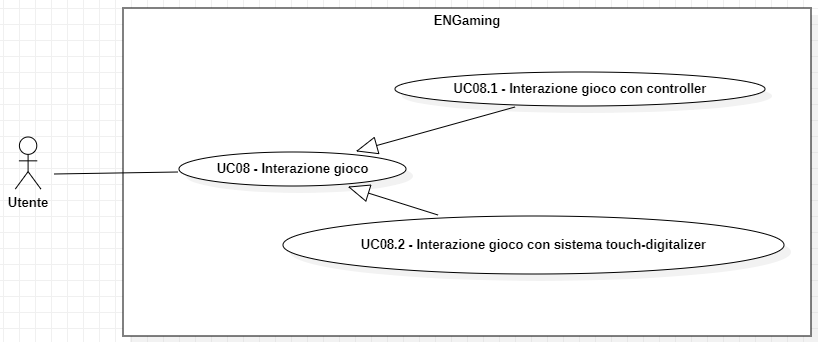
\includegraphics[width=400pt]{images/usecase/UC08.png}
    \caption{Diagramma dei casi d'uso per l'interazione con un gioco}
    \label{fig:UC08}
\end{figure}
\begin{itemize}
    \item Attore principale: Utente
    \item Pre-condizioni: l'utente vuole eseguire una determinata azione nel gioco.
    \item Post-condizioni: l'utente ha eseguito l'azione nel gioco.
    \item Scenario principale: \begin{itemize}
        \item L'utente esegue un azione attraverso l'interfaccia del gioco.
        \item Il sistema riceve l'input dell'interfaccia dal device e lo elabora.
        \item Il sistema prende il dato elaborato e lo manda al gioco.
    \end{itemize}
\end{itemize}

\subsection{UC08.1 - Interazione gioco con controller}
\begin{itemize}
    \item Attore principale: Utente
    \item Pre-condizioni: l'utente vuole eseguire una determinata azione nel gioco.
    \item Post-condizioni: l'utente ha eseguito l'azione nel gioco.
    \item Scenario principale: \begin{itemize}
        \item L'utente preme un pulsante nel controller.
        \item Il sistema riceve l'input del controller dal device e lo elabora.
        \item Il sistema prende il dato elaborato e lo manda al gioco.
    \end{itemize}
\end{itemize}

\subsection{UC08.2 - Interazione gioco con sistema touch-digitalizer}
\begin{itemize}
    \item Attore principale: Utente
    \item Pre-condizioni: l'utente vuole eseguire una determinata azione nel gioco.
    \item Post-condizioni: l'utente ha eseguito l'azione nel gioco.
    \item Scenario principale: \begin{itemize}
        \item L'utente esegue una gesture, ovvero un gesto, nel gioco.
        \item Il sistema riceve l'input del gesto dal device e lo elabora.
        \item Il sistema prende il dato elaborato e lo manda al gioco.
    \end{itemize}
\end{itemize}

\subsection{UC09 - Pausa del gioco}
\begin{figure}[h]
    \centering
    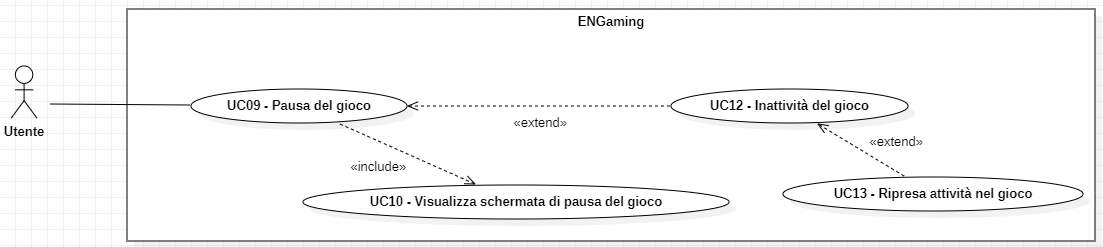
\includegraphics[width=400pt]{images/usecase/UC09.png}
    \caption{Diagramma dei casi d'uso per la pausa di un gioco}
    \label{fig:UC09}
\end{figure}
\begin{itemize}
    \item Attore principale: Utente
    \item Pre-condizioni: l'utente vuole mettere in pausa il gioco.
    \item Post-condizioni: il gioco è in stato di pausa.
    \item Scenario principale: \begin{itemize}
        \item L'utente preme l'apposito pulsante di pausa.
        \item Il sistema riceve l'input dal device e mette in pausa il gioco.
        \item L'utente visualizza una pagina che informa dello stato di pausa del gioco.
    \end{itemize}
    \item Include: \begin{itemize}
        \item UC10 - Visualizza schermata di pausa del gioco
    \end{itemize}
    \item Estensioni: \begin{itemize}
        \item UC12 - Inattività del gioco
    \end{itemize}
\end{itemize}
\newpage
\subsection{UC10 - Visualizza schermata di pausa del gioco}
\begin{figure}[h]
    \centering
    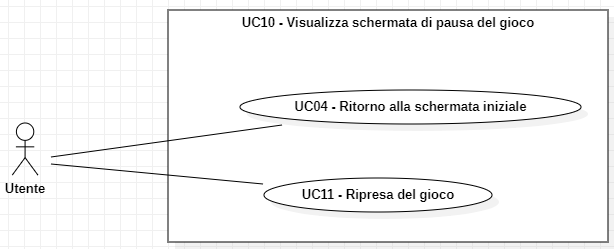
\includegraphics[width=400pt]{images/usecase/UC10.png}
    \caption{Diagramma dei casi d'uso per la schermata di pausa}
    \label{fig:UC10}
\end{figure}
\begin{itemize}
    \item Attore principale: Utente
    \item Pre-condizioni: L'utente ha messo in pausa il gioco.
    \item Post-condizioni: L'utente è informato dello stato di pausa del gioco.
    \item Scenario principale: \begin{itemize}
        \item L'utente visualizza una pagina che informa dello stato di pausa del gioco. La pagina contiene una scritta che avvisa l'utente dello stato di pausa del gioco e due pulsanti. Il primo pulsante permette di ricominciare a giocare, togliendo il gioco dallo stato di pausa, mentre il secondo permette di chiudere il gioco e tornare alla schermata iniziale.
    \end{itemize}
    \item Include: \begin{itemize}
        \item UC04 - Ritorno alla schermata iniziale
        \item UC11 - Ripresa del gioco
    \end{itemize}
\end{itemize}

\subsection{UC11 - Ripresa del gioco}
\begin{itemize}
    \item Attore principale: Utente
    \item Pre-condizioni: il gioco è in stato di pausa.
    \item Post-condizioni: il gioco è uscito dallo stato di pausa e l'utente può continuare a giocare.
    \item Scenario principale: \begin{itemize}
        \item L'utente preme l'apposito pulsante di ripresa del gioco.
        \item Il sistema riceve l'input dal device e toglie lo stato di pausa dal gioco.
    \end{itemize}
\end{itemize}

\subsection{UC12 - Inattività nel gioco}
\begin{itemize}
    \item Attore principale: Utente
    \item Pre-condizioni: l'utente non sta eseguendo alcuna attività sul gioco.
    \item Post-condizioni: il sistema visualizza la schermata iniziale.
    \item Scenario principale: \begin{itemize}
        \item Dopo 10 secondi dall'ultimo input, il sistema avvia un cronometro di quattro minuti.
        \item Al termine del cronometro, il sistema chiude il gioco e torna alla schermata iniziale.
    \end{itemize}
    \item Estensioni: \begin{itemize}
        \item UC13 - Ripresa attività nel gioco
    \end{itemize}
\end{itemize}

\subsection{UC13 - Ripresa attività nel gioco}
\begin{itemize}
    \item Attore principale: Utente
    \item Pre-condizioni: l'utente non sta eseguendo alcuna attività sul gioco.
    \item Post-condizioni: l'utente ha eseguendo un'attività sul gioco.
    \item Scenario principale: \begin{itemize}
        \item Dopo 10 secondi dall'ultimo input, il sistema avvia un cronometro di quattro minuti.
        \item L'utente esegue un'attività sul gioco prima dello scadere del cronometro.
        \item Il sistema interrompe il cronometro e lo riporta alla durata iniziale.
    \end{itemize}
\end{itemize}
\newpage
\subsection{UC14 - Inserimento nuovo record}
\begin{figure}[h]
    \centering
    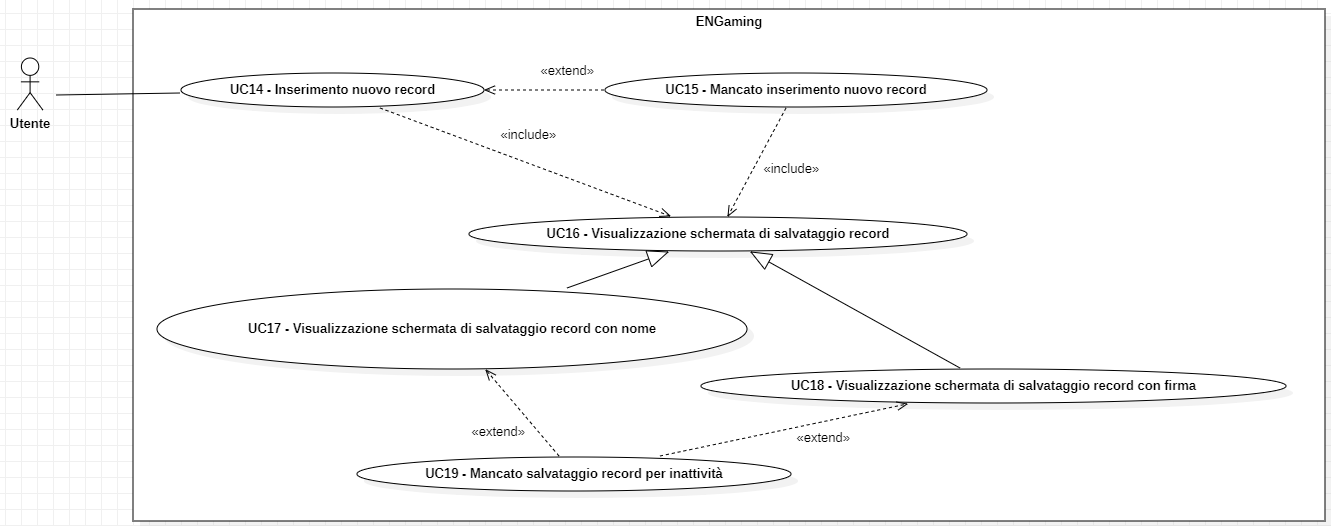
\includegraphics[width=410pt]{images/usecase/UC14.png}
    \caption{Diagramma dei casi d'uso per l'inserimento di un nuovo record}
    \label{fig:UC14}
\end{figure}
\begin{itemize}
    \item Attore principale: Utente
    \item Pre-condizioni: l'utente chiude il gioco, ed ha effettuato un nuovo record.
    \item Post-condizioni: il sistema ha memorizzato il record effettuato dall'utente.
    \item Scenario principale: \begin{itemize}
        \item L'utente visualizza una schermata per informarlo della creazione di un nuovo record.
        \item Tramite la schermata, l'utente seleziona il metodo di salvataggio del record che più preferisce.
        \item Il sistema riceve il dato inserito dall'utente e memorizza il record.
    \end{itemize}
    \item Include: \begin{itemize}
        \item UC16 - Visualizzazione schermata di salvataggio record
    \end{itemize}
    \item Estensioni: \begin{itemize}
        \item UC15 - Mancato inserimento nuovo record 
    \end{itemize}
\end{itemize}

\subsection{UC15 - Mancato inserimento nuovo record}
\begin{itemize}
    \item Attore principale: Utente
    \item Pre-condizioni: l'utente ha effettuato un nuovo record in un gioco, ma non vuole salvarlo.
    \item Post-condizioni: il sistema non ha memorizzato il record effettuato dall'utente.
    \item Scenario principale: \begin{itemize}
        \item L'utente visualizza una schermata per informarlo della creazione di un nuovo record.
        \item Tramite la schermata, l'utente seleziona la volontà di non salvare il record effettuato.
        \item Il sistema scarta i dati relativi al record e non lo memorizza.
    \end{itemize}
    \item Include: \begin{itemize}
        \item UC16 - Visualizzazione schermata di salvataggio record
    \end{itemize}
\end{itemize}

\subsection{UC16 - Visualizzazione schermata di salvataggio record}
\begin{itemize}
    \item Attore principale: Utente
    \item Pre-condizioni: l'utente ha effettuato un nuovo record in un gioco.
    \item Post-condizioni: l'utente sta visualizzando la schermata relativa al salvataggio del record.
    \item Scenario principale: \begin{itemize}
        \item L'utente visualizza la schermata che lo informa della creazione di un nuovo record, e ne propone il salvataggio. Questa schermata, oltre a riportare il punteggio del record, propone tre opzioni: il salvataggio del record tramite nome, il salvataggio del record tramite firma e il non salvataggio del record.
    \end{itemize}
\end{itemize}

\subsection{UC17 - Visualizzazione schermata di salvataggio record con nome}
\begin{itemize}
    \item Attore principale: Utente
    \item Pre-condizioni: l'utente vuole salvare il record con il proprio nome.
    \item Post-condizioni: l'utente ha inserito il proprio nome correttamente.
    \item Scenario principale: \begin{itemize}
        \item L'utente visualizza la schermata di salvataggio tramite nome. Il nome può essere inserito tramite due pulsanti per carattere, ognuno dei quali passa al carattere precedente o al successivo. Una volta che l'utente è soddisfatto, può premere l'apposito pulsante per il salvataggio del nome.
    \end{itemize}
    \item Estensioni: \begin{itemize}
        \item UC19 - Mancato salvataggio record per inattività
    \end{itemize}
\end{itemize}


\subsection{UC18 - Visualizzazione schermata di salvataggio record con firma}
\begin{itemize}
    \item Attore principale: Utente
    \item Pre-condizioni: l'utente vuole salvare il record con la propria firma.
    \item Post-condizioni: l'utente ha inserito la propria firma correttamente.
    \item Scenario principale: \begin{itemize}
        \item L'utente visualizza la schermata di salvataggio tramite firma. La firma può essere inserita sia tramite l'utilizzo del touch screen, quindi firmando con il dito, sia tramite l'utilizzo del digitalizer. Una volta che l'utente è soddisfatto, può premere l'apposito pulsante per il salvataggio della firma.
    \end{itemize}
    \item Estensioni: \begin{itemize}
        \item UC19 - Mancato salvataggio record per inattività
    \end{itemize}
\end{itemize}

\subsection{UC19 - Mancato salvataggio record per inattività}
\begin{itemize}
    \item Attore principale: Utente
    \item Pre-condizioni: l'utente non sta eseguendo alcuna attività  sulla schermata di salvataggio record.
    \item Post-condizioni: il record non viene salvato nel sistema.
    \item Scenario principale: \begin{itemize}
        \item Dopo dieci secondi dall'ultima interazione, il sistema avvia un cronometro di quattro minuti.
        \item Al termine del cronometro, il sistema chiude la schermata di salvataggio record, non salva il record e torna alla schermata iniziale.
    \end{itemize}
\end{itemize}
\newpage
\section{Requisiti}
In questa sezione vengono elencati i requisiti analizzati per l'applicativo.
Le tabelle, suddivide per tipologia di requisito, forniscono le seguenti informazioni:
\begin{itemize}
    \item \textbf{Codice}, che indica la tipologia di requisito (tra F=funzionale, Q=qualità e V=vincolo) e il numero del requisito;
    \item \textbf{Requisito}, dove si indica il requisito vero e proprio;
    \item \textbf{Tipologia}, ovvero se il requisito indicato è obbligatorio oppure opzionale;
    \item \textbf{Caso d'uso} di riferimento (solo per i requisiti funzionali).
\end{itemize}
\subsection{Requisiti funzionali}
\begin{longtable}{|c|c|c|c|}
    \hline
    \thead{Codice}&\thead{Requisito}&\thead{Tipologia}&\thead{Caso d'uso}\\
    \hline
    RF01&\makecell{Dev'essere possibile \\ visualizzare la lista \\ di giochi disponibili}&Obbligatorio&UC01,UC02\\
    \hline
    RF02&\makecell{Dev'essere possibile \\ utilizzare dei pulsanti per \\ visualizzare le icone nascoste}&Obbligatorio&UC02\\
    \hline
    RF03&\makecell{Dev'essere possibile \\ toccare le icone presenti nella \\ schermata iniziale}&Obbligatorio&UC01,UC02,UC03\\
    \hline
    RF04&\makecell{Dev'essere possibile \\ visualizzare le informazioni \\ relative a un singolo gioco}&Obbligatorio&UC02.1\\
    \hline
    RF05&\makecell{Dev'essere possibile \\ visualizzare la lista \\ dei record globali}&Obbligatorio&UC03\\
    \hline
    RF06&\makecell{Dev'essere possibile \\ visualizzare la lista \\ dei record per ogni gioco presente}&Obbligatorio&UC03\\
    \hline
    RF07&\makecell{Dev'essere possibile \\ utilizzare dei pulsanti \\ per visualizzare i record nascosti}&Obbligatorio&UC03\\
    \hline
    RF08&\makecell{Dev'essere possibile \\ visualizzare le informazioni \\ relative a un singolo record}&Obbligatorio&UC03.1,UC03.2\\
    \hline
    RF09&\makecell{Dev'essere possibile \\ ritornare alla schermata iniziale}&Obbligatorio&UC04\\
    \hline
    RF10&\makecell{Dev'essere possibile \\ avviare un gioco}&Obbligatorio&UC05\\
    \hline
    RF11&\makecell{Dev'essere possibile \\ visualizzare una pagina \\ di caricamento}&Obbligatorio&UC06\\
    \hline
    RF12&\makecell{La pagina di caricamento \\ dev'essere visibile \\ per almeno quattro secondi}&Obbligatorio&UC06\\
    \hline
    RF13&\makecell{Dev'essere possibile \\ l'utilizzo di \\ un controller virtuale}&Obbligatorio&UC07.1\\
    \hline
    RF14&\makecell{Il controller \\ deve avere nove tasti}&Obbligatorio&UC07.1\\
    \hline
    RF15&\makecell{Il controller \\ non deve richiede \\ l'impugnatura del device utilizzato}&Obbligatorio&UC07.1\\
    \hline
    RF16&\makecell{Dev'essere possibile \\ giocare utilizzando le dita delle mani}&Obbligatorio&UC07.2\\
    \hline
    RF17&\makecell{Dev'essere possibile \\ giocare utilizzando il digitalizer}&Obbligatorio&UC07.2\\
    \hline
    RF18&\makecell{Il pulsante di pausa \\ deve occupare il meno possibile \\ l'area di gioco}&Obbligatorio&UC07.2\\
    \hline
    RF19&\makecell{Dev'essere possibile \\ interagire con un gioco \\ attraverso il controller}&Obbligatorio&UC08.1\\
    \hline
    RF20&\makecell{Dev'essere possibile \\ interagire con un gioco \\ attraverso le dita delle mani}&Obbligatorio&UC8.2\\
    \hline
    RF21&\makecell{Dev'essere possibile \\ interagire con un gioco \\ attraverso il digitalizer}&Obbligatorio&UC8.2\\
    \hline
    RF22&\makecell{Dev'essere possibile \\ mettere in pausa \\ un gioco}&Obbligatorio&UC09\\
    \hline
    RF23&\makecell{Il sistema deve avvisare \\ quando un gioco \\ è in pausa}&Obbligatorio&UC09,UC10\\
    \hline
    RF24&\makecell{Dev'essere possibile \\ far ripartire un gioco \\ dopo la pausa}&Obbligatorio&UC10,11\\
    \hline
    RF25&\makecell{Dev'essere possibile \\ chiudere un gioco e tornare \\ alla schermata iniziale}&Obbligatorio&UC10,UC04\\
    \hline
    RF26&\makecell{Il sistema deve tornare \\ alla schermata iniziale \\ dopo quattro minuti d'inattività}&Obbligatorio&UC12,UC19\\
    \hline
    RF27&\makecell{Il sistema deve far partire \\ il cronometro d'inattività \\ dopo dieci secondi dall'ultimo input}&Obbligatorio&UC12,UC19\\
    \hline
    RF28&\makecell{Il sistema deve interrompere \\ il cronometro d'inattività all'azione \\ dell'utente, prima del suo scadere}&Obbligatorio&UC13\\
    \hline
    RF29&\makecell{Dev'essere possibile \\ memorizzare un nuovo record}&Obbligatorio&UC14\\
    \hline
    RF30&\makecell{L'utente deve poter scegliere \\ se salvare o no \\ il record effettuato}&Obbligatorio&UC14,UC15,UC16\\
    \hline
    RF31&\makecell{L'utente deve visualizzare \\ la schermata dove decidere \\ se salvare un record}&Obbligatorio&UC16\\
    \hline
    RF32&\makecell{L'utente deve poter salvare \\ il record \\ tramite il suo nome}&Obbligatorio&UC17\\
    \hline
    RF33&\makecell{L'utente deve poter \\ inserire il suo nome}&Obbligatorio&UC17\\
    \hline
    RF34&\makecell{L'utente deve poter salvare \\ il record \\ tramite la sua firma}&Opzionale&UC18\\
    \hline
    RF35&\makecell{L'utente deve poter \\ inserire la sua firma}&Opzionale&UC18\\
    \hline
    RF36&\makecell{Il sistema non deve \\ salvare il record \\ in caso d'inattività}&Obbligatorio&UC19\\
    \hline
    \caption{Tabella dei requisiti funzionali}
\end{longtable}
\subsection{Requisiti di qualità}
    \begin{longtable}{|c|c|c|c|} 
        \hline
        \thead{Codice}&\thead{Requisito}&\thead{Tipologia}\\
        \hline
        RQ01 &\makecell{Dev'essere fornita la documentazione necessaria \\ per l'utilizzo del prodotto} & Obbligatorio\\
        \hline
        RQ02 & \makecell{Dev'essere fornita la documentazione necessaria \\ per la manutenzione del prodotto} & Obbligatorio\\ 
        \hline
        RQ03 & \makecell{Il prodotto dev'essere versionato e pubblicato \\ sulle piattaforme aziendali} & Obbligatorio\\
        \hline
        \caption{Tabella dei requisiti di qualità}
    \end{longtable}
\subsection{Requisiti di vincolo}
\begin{longtable}{|c|c|c|c|}
    \hline
    \thead{Codice}&\thead{Requisito}&\thead{Tipologia}\\
    \hline
    RV01 & \makecell{L'interfaccia grafica del prodotto \\ dev'essere sviluppata utilizzando \\ i linguaggi HTML, CSS, JavaScript e TypeScript} & Obbligatorio\\
    \hline
    RV02 & \makecell{L'interfaccia grafica del prodotto \\ dev'essere sviluppata utilizzando \\ il framework Angular} & Obbligatorio\\
    \hline
    RV03 & \makecell{L'interfaccia grafica del prodotto \\ dev'essere sviluppata utilizzando \\ il framework Electron} & Obbligatorio\\
    \hline
    RV04 & \makecell{Il prodotto dev'essere utilizzabile \\ attraverso il device ENSign 11} & Obbligatorio\\
    \hline
    RV05 & \makecell{Il prodotto deve utilizzare \\ il linguaggio C++ per la ricezione dei dati dal device} & Obbligatorio\\
    \hline
    RV06 & \makecell{Il prodotto dev'essere utilizzabile \\ senza impugnare il device} & Obbligatorio\\
    \hline
    RV07 & \makecell{Il prodotto dev'essere utilizzabile \\ attraverso il sistema touch screen del device} & Obbligatorio\\
    \hline
    RV08 & \makecell{Il prodotto dev'essere utilizzabile \\ attraverso il digitalizer presente nel device} & Obbligatorio\\
    \hline
    \caption{Tabella dei requisiti di vincolo}
\end{longtable}